\section{PHÂN TÍCH CÂU 3}
\addcontentsline{toc}{section}{\numberline {} PHÂN TÍCH CÂU 3}
\setcounter{section}{3}
* \textbf{Truy cập link github để có thể xem code tốt nhất:}  \url{https://github.com/DoTienThanh325/Big_exercise/tree/main/Problem%203}
\subsection{Ý tưởng làm bài}
Sử dụng thuật toán K-means để phân chia các nhóm cầu thủ sử dụng phương pháp Elbow để tìm số cụm phân chia. Sử dụng PCA để giảm chiều dữ liệu xuống và vẽ lại biểu đồ phân cụm.
\subsection{Phân tích code câu 3}
\begin{figure}[H]
    \centering
    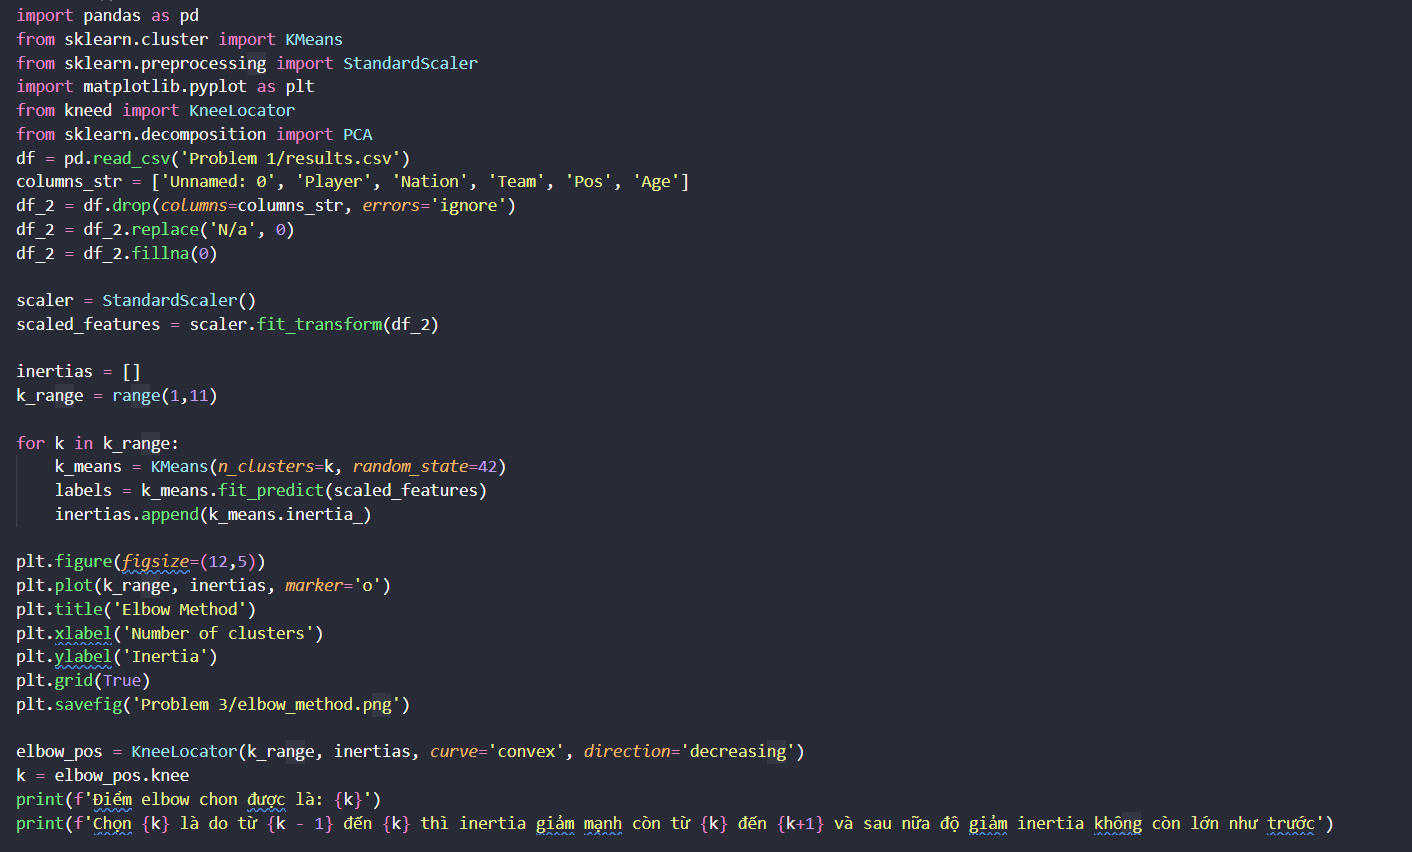
\includegraphics[width=1\linewidth]{img/3_1.png}
\end{figure}
- Đoạn code: 
\begin{verbatim}
columns_str = ['Unnamed: 0', 'Player', 'Nation', 'Team', 'Pos', 'Age']
df_2 = df.drop(columns=columns_str, errors='ignore')
df_2 = df_2.replace('N/a', 0)
df_2 = df_2.fillna(0)   
\end{verbatim}
Xứ lý dữ liệu gần giống câu 2 nhưng không trực tiếp lấy cột có dạng số mà loại bỏ các cột có dạng chữ. Thay tất cả 'N/a' và giá trị NaN sang giá trị 0.\\
- Chuẩn hóa dữ liệu để áp dụng các hàm sẵn có cho thuật toán k\_means:
\begin{verbatim}
    scaler = StandardScaler()
    scaled_features = scaler.fit_transform(df_2)
\end{verbatim}
- Khởi chạy đoạn code theo phương pháp elbow:
\begin{verbatim}
    inertias = []
    k_range = range(1,11)

    for k in k_range:
        k_means = KMeans(n_clusters=k, random_state=42)
        labels = k_means.fit_predict(scaled_features)
        inertias.append(k_means.inertia_)
\end{verbatim}
\begin{itemize}
    \item Khởi tạo danh sách \textbf{inertias}: Dùng để lưu trữ giá trị inertia cho mỗi số
    lượng cụm k.
    \item Lặp qua các giá trị \textbf{k} từ 1 đến 10 (với \textbf{range(1,11)}):
    \begin{itemize}[label=$\circ$]
        \item Đối với mỗi giá trị \textbf{k}, ta tạo một đối tượng \textbf{KMeans} và áp dụng phương thức \textbf{fit\_predict} để phân cụm dữ liệu.
        \item \textbf{fit\_predict} sẽ trả về labels (nhãn cụm cho từng điểm dữ liệu) và cập nhật đối tượng \textbf{k\_means}.
    \end{itemize}
    \item Lưu giá trị inertia vào danh sách \textbf{inertias}: Inertia là tổng bình phương khoảng cách từ các điểm đến tâm của cụm gần nhất, được tính qua \textbf{ k\_means.inertia\_}.
\end{itemize}
- Tiếp theo thực hiện vẽ biểu đồ Elbow method với trục x là số nhóm còn y là Inertia, có thể dựa vào biểu đồ tìm elbow hoặc có thể dùng thư viện knee để chính xác nhất:
\begin{verbatim}
    plt.figure(figsize=(12,5))
    plt.plot(k_range, inertias, marker='o')
    plt.title('Elbow Method')
    plt.xlabel('Number of clusters')
    plt.ylabel('Inertia')
    plt.grid(True)
    plt.savefig('Problem 3/elbow_method.png')
    
    elbow_pos = KneeLocator(k_range, inertias, curve='convex',direction=
    'decreasing')
    k = elbow_pos.knee
    print(f'Điểm elbow chon được là: {k}')
\end{verbatim}
\begin{figure}[H]
    \centering
    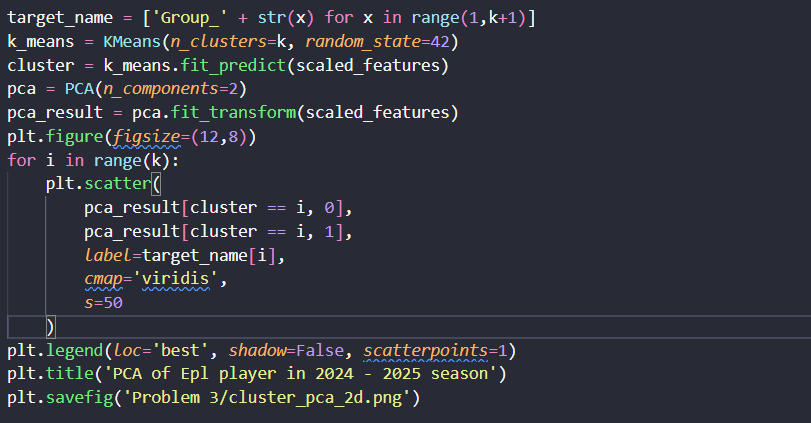
\includegraphics[width=1\linewidth]{img/3-2.png}
\end{figure}
- Tạo tên nhóm cụm (\textbf{target\_name}):
\begin{itemize}
    \item Tạo một danh sách tên nhóm có dạng ['Group\_1', 'Group\_2', ..., 'Group\_k'], với k là số cụm.
\end{itemize}
- Áp dụng \textbf{KMeans}:
\begin{itemize}
    \item \textbf{k\_means = KMeans(n\_clusters=k, random\_state=42)}: Khởi tạo đối tượng KMeans với số cụm \textbf{k}.
    \item \textbf{cluster = k\_means.fit\_predict(scaled\_features)}: Dự đoán nhóm cho các mẫu trong \textbf{scaled\_features} và lưu kết quả vào cluster.
\end{itemize}
- Áp dụng PCA:
\begin{itemize}
    \item \textbf{pca = PCA(n\_components=2)}: Khởi tạo đối tượng PCA để giảm chiều dữ liệu xuống 2 chiều.
    \item \textbf{pca\_result = pca.fit\_transform(scaled\_features)}: Áp dụng PCA lên dữ liệu chuẩn hóa \textbf{scaled\_features}.
\end{itemize}
- Vẽ biểu đồ phân cụm:
\begin{itemize}
    \item \textbf{plt.scatter()}: Vẽ các điểm trên biểu đồ 2D với màu sắc khác nhau cho từng nhóm cụm (cluster == i).
    \item \textbf{label=target\_name[i]}: Đặt tên cho mỗi nhóm tương ứng với các cụm.
    \item \textbf{plt.legend()}: Thêm chú thích vào biểu đồ.
    \item \textbf{plt.savefig()}: Lưu biểu đồ vào tệp \textbf{cluster\_pca\_2d.png}.
\end{itemize}